%%%%%%%%%%%%%%%%%%%%%%%%%%%%%%%%%%%%%%%%%%%%%%%%%%%%%%%%%%%%%%%%%%%%%
\documentclass{anstrans}
%
%  various packages that you may wish to activate for usage 
\usepackage{graphicx}
\usepackage{tabls}
\usepackage{hyperref}
\hypersetup{breaklinks=true, linkcolor=black, citecolor=black,
  urlcolor=black, colorlinks=true, pdftitle={PyNE Progress Report}}
\usepackage{listings}
\usepackage{booktabs}
%

%General Short-Cut Commands
\newcommand{\superscript}[1]{\ensuremath{^{\textrm{#1}}}}
\newcommand{\subscript}[1]{\ensuremath{_{\textrm{#1}}}}
%\newcommand{\nuc}[2]{\superscript{#2}{#1}}
\newcommand{\nuc}[2]{{#1}-{#2}}
\newcommand{\ith}[0]{$i^{\mbox{th}}$ }
\newcommand{\jth}[0]{$j^{\mbox{th}}$ }
\newcommand{\kth}[0]{$k^{\mbox{th}}$ }
\newcommand{\us}[0]{$\mu$s }

% New definition of square root:
% it renames \sqrt as \oldsqrt
\let\oldsqrt\sqrt
% it defines the new \sqrt in terms of the old one
\def\sqrt{\mathpalette\DHLhksqrt}
\def\DHLhksqrt#1#2{%
\setbox0=\hbox{$#1\oldsqrt{#2\,}$}\dimen0=\ht0
\advance\dimen0-0.2\ht0
\setbox2=\hbox{\vrule height\ht0 depth -\dimen0}%
{\box0\lower0.4pt\box2}}



\title{PyNE Progress Report}

\author{Anthony~Scopatz$^1$, Elliott~D.~Biondo$^1$, 
        Carsten Brachem$^2$, John Xia$^3$, 
        Paul P. H. Wilson$^1$}

\institute{$^1$ The University of Wisconsin-Madison, 1415 Engineering Drive, Madison, WI 53706, USA \\
  $^2$ Technische Universit\"at Dresden, Helmholtzstr. 10 01069 Dresden, Germany\\
  $^3$ The University of Chicago, 5747 S. Ellis Ave, Jones 311, Chicago, IL  60637}
\email{scopatz@wisc.edu}


%%%%%%%%%%%%%%%%%%%%%%%%%%%%%%%%%%%%%%%%%%%%%%%%%%%%%%%%%%%%%%%%%%%%%
%
%   BEGIN DOCUMENT
%
%%%%%%%%%%%%%%%%%%%%%%%%%%%%%%%%%%%%%%%%%%%%%%%%%%%%%%%%%%%%%%%%%%%%%
\begin{document}


% \begin{abstract}
% %\raggedright
% 
% PyNE, the nuclear engineering toolkit, has recently received several major
% feature additions.  These include support for reading and writing PyNE materials 
% as ALARA materials.  Additionally, MOAB has been selected as the PyNE mesh package
% and MCNP MESHTAL file handlers are available.  Furthermore, MCNP PTRAC files may now
% easily be converted to an HDF5 file.  Lastly, an ENDF reader has been written and 
% optimized.
% 
% \emph{Key Words}: PyNE, MCNP, ENDF
% \end{abstract}
% 
% \setlength{\baselineskip}{11pt}


\section{Introduction}
\label{sec:intro}

PyNE is a suite of free and open source (BSD licensed) tools to aid in 
computational nuclear science \& engineering. PyNE seeks to provide native 
implementations of common nuclear algorithms, as well as Python bindings and 
I/O support for industry standard nuclear codes.  In recent months, the development 
of PyNE has largely focused on feature 
enhancements for external tools.  These additions include interfacing with 
codes such as ALARA, MCNP, MOAB as well as the ENDF cross section data
file format.

\section{Enhanced Capabilities}

\subsection{Material Handling}

Improvements to material handling have been added to the \texttt{pyne.material}
and \texttt{pyne.mcnp} modules. A new attribute was added to the
\texttt{pyne.material.Material} class in order to store material metadata (e.g.,
material name, the source of the material definition, comments).
\texttt{Material} class methods were added to write material definitions in MCNP
and ALARA \cite{wilson_alara:_1999} input file formats.  These material
definitions are prepended by comments containing the aforementioned metadata. 

In addition, a function was added to \texttt{pyne.mcnp} to read MCNP input files and
create \texttt{Material} objects for each material specified in the file. This
function can parse formatted comments in MCNP input files in order to
populate the metadata fields of each \texttt{Material} object.

Moreover a new class called \texttt{pyne.material.MultiMaterial} was added.  This
represents collections of materials along with corresponding mass or
volume fractions.  Class methods allow for mixing of these collections by mass
or volume fraction in order to create \texttt{ Material} objects.

\subsection{MCNP Support}

Two classes have been added to the \texttt{pyne.mcnp} module in order to store
MCNP data on Mesh Oriented datABase (MOAB) meshes \cite{tautges_moab:_2004}.
Storing data on MOAB meshes has numerous benefits including access to preexisting
mesh and data manipulation capabilities and easy visualization options. These
meshes are created using PyTAPS \cite{pytaps}, the Python interface to MOAB.
As an example of MOAB mesh visualization may be seen in Figure \ref{moabexp}.
This visualization was produced with the yt analysis package \cite{ytpaper}.

\begin{figure}[htbp]
\begin{center}
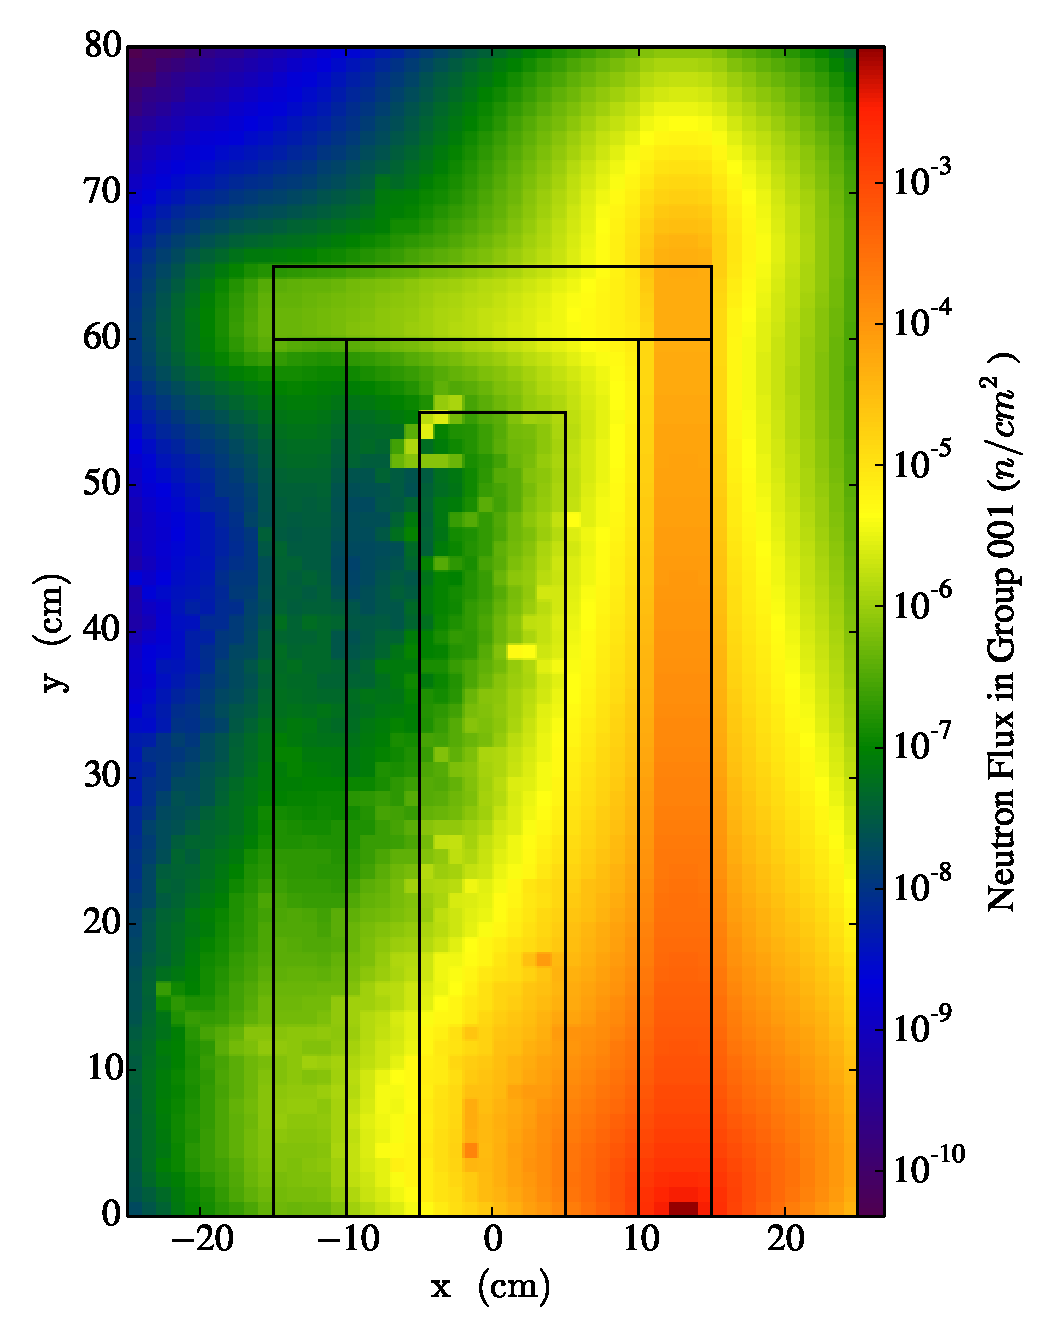
\includegraphics[scale=0.35]{moab_example.eps}
\end{center}
\caption{A MOAB mesh which displays the neutron mesh tally results from a U-shaped 
         duct streaming problem with a 14 MeV isotropic neutron source.}
\label{moabexp}
\end{figure}

First, the \texttt{pyne.mcnp.Wwinp} class represents all information contained in a
single Cartesian MCNP WWINP file.   Such files contain a set of weight window lower
bounds for neutrons, photons, or both. The weight window lower bounds are
stored on a structured MOAB mesh attribute. In addition to class methods that
read-in and write-out MCNP WWINP files, \texttt{Wwinp} objects can be created
directly from MOAB meshes tagged with weight window lower bounds. This will
facilitate the future implementation of weight window generation schemes (e.g.,
MAGIC \cite{davis_comparison_2011}, CADIS \cite{haghighat_monte_2003}) within
PyNE.

Next, the \texttt{pyne.mcnp.Meshtal} class represents the information from a 
Cartesian MCNP MESHTAL file. These files may contain multiple neutron and/or 
photon mesh
tallies.  Tally results and relative errors are stored on structured MOAB
meshes. A dictionary attribute allows key-value access to these meshes using
tally numbers (i.e., 4, 14, 24, ...) as keys. Other methods allow for the
addition and subtraction of tally values for different mesh tallies.

Another addition to PyNE's MCNP capabilities is the ability to read and
process particle track (PTRAC) files. The \texttt{PTRAC} card allows MCNP
users to record complete particle histories for selected events. However,
the custom binary file format used to save the particle tracks is cumbersome
to work with and varies in details, depending on system architecture or
how MCNP was compiled. The available plain text format for particle
tracks is unfeasible due to the large size of the generated files and the
poor speed associated with processing plain text files. Therefore, only
binary PTRAC files are supported by PyNE at this moment.

The \texttt{pyne.mcnp.PtracReader} class takes care of all the details
involved in reading particle track files and offers a simple interface
for reading event information and metadata associated with the run.
It also has a built-in function to write the particle tracks directly
to a file in the well-known HDF5 format \cite{hdf5}.
A small command line utility program called \texttt{ptrac\_to\_hdf5} is
provided to make converting PTRAC files as convenient as possible
for the common use case. Listing \ref{fig_ptractohdf5} shows the usage
description of the conversion program.

\begin{figure*}[htbp]
\begin{lstlisting}[frame=single,basicstyle=\scriptsize\ttfamily,label=fig_ptractohdf5,caption=Usage description of the PTRAC to HDF5 command line utility.]
usage: ptrac_to_hdf5 [-h] [-n TABLE_NAME] [-t TABLE_TITLE] [-s] ptrac_file hdf5_file

write the contents of a MCNP PTRAC file to a HDF5 table

positional arguments:
  ptrac_file            MCNP PTRAC file to read from
  hdf5_file             HDF5 file to write to (will be created if it does not exist)

optional arguments:
  -h, --help            show this help message and exit
  -n TABLE_NAME, --table-name TABLE_NAME
                        name of the HDF5 table (default is "ptrac")
  -t TABLE_TITLE, --table-title TABLE_TITLE
                        title of the HDF5 table (default is "Ptrac data")
  -s, --show-progress   show progress indicator
\end{lstlisting}
\end{figure*}

\subsection{ENDF Reader Support}

A significant improvement to the PyNE toolkit has been the development of 
a fully fledged ENDF \cite{herman2009endf} reader.  This parser is capable 
of handling all ENDF files and evaluations. The performance of the reader is 
extraordinarily fast due to a number of innovative optimizations.

At the top-most level a \texttt{Library} class is defined in the \texttt{pyne.endf}
module.  This module is itself written in the Cython language \cite{behnel2010cython}.
The Cython compiler itself acts as a code-generation and optimization pass whereby
Python code becomes non-idomatic C/C++.  Furthermore this reader implements a
`lazy' strategy that only loads data sets into memory upon request rather 
than upon initialization.  This enables evaluations in a single physical file to be 
read independently.  This is a huge usability boon to interactive exploration of 
cross section data and decreases application start up times.

However, the most ubiquitous speed up is in terms of converting the string
data values in the file to machine floats.  The data values stored in ENDF 
are not in an encoding compliant with
most modern programming languages float literals. Thus the built-in tools do not 
handle ENDF-type floats natively.  However, the ENDF format does have a couple
of advantages.  It elides the `e' separator between the exponent and mantissa and
relies on the `+' and `-' characters.  This reduces the overall storage size.
Furthermore, the string literal is a fixed 11 characters long. The first character
is always a `+' or `-' or space.  The third character is always the floating point.
There are only two exponent characters. All other characters are digits.  
For example, ``\texttt{-3.28559+12}" is a valid number in the ENDF format.

The predictability of this format allows for several optimizations.  A na\"{i}ve 
implementation would simply add the missing exponent `e' character to create
a standards compliant float string and then call the \texttt{atof()} function.  
However, this does not leverage the known width of ENDF or the known position of
the non-digit characters.  Hence a C++ function named \texttt{endftod()} was 
created which takes advantage of this \emph{a priori} information.  
Table \ref{endftod} compares the average runtimes. The custom algorithm is nearly 
five times faster on the most-called routine when parsing ENDF files.

\begin{table}
\centering
\caption{ENDF Float Conversion Comparison}
\label{endftod}
{\small
\begin{tabular}[htbp]{lcc}
\toprule
\textbf{Implementation} & \textbf{Average Run Time [ns]} & \textbf{Speed Up} \\
\midrule
Na\"{i}ve Python, \texttt{float()} & 539 & 1.0 \\
Na\"{i}ve C, \texttt{atof()} & 229 & 2.3 \\
PyNE, \texttt{endftod()} & 114 & 4.7 \\
\bottomrule
\end{tabular}
}
\end{table}

\begin{lstlisting}[language=Python,basicstyle=\scriptsize\ttfamily,frame=single,caption=ENDF Reader API,label=endfapi]
from pyne.endf import Library
u235 = Library("U235-VII.txt")
xs_data = u235.get_xs(922350, 16)[0]
\end{lstlisting}

\begin{figure}[htbp]
  \centering
  \includegraphics[width=0.5\textwidth]{u235_2n.eps}
  \caption{U-235 (n, 2n) Cross Section from ENDF Evaluation}
  \label{u235}
\end{figure}

As an example of the ENDF reader usage, the following code in Listing \ref{endfapi} 
displays the top-level interface required to load a data set.  Figure \ref{u235} 
then displays the data garnered in this way.  This reader has also
been exposed as a cross section data source available in the \texttt{pyne.xs} 
sub-package.


\section{Conclusions \& Future Work}
\label{sec:conc}

The building of the PyNE-based tools presented above demonstrates major 
accomplishments with respect
to interfacing with external tools.  Both ENDF and MCNP are keystones of 
nuclear engineering software development.  The PyNE project will continue to create 
free and open source tools that easily interface the plethora of choices available 
in nuclear engineering and scientific computing. 

\bibliographystyle{ans}
\bibliography{refs}

\end{document}
